\documentclass[tikz,border=10pt]{standalone}
\usepackage{amsmath}
\usepackage{tikz}
\usetikzlibrary{arrows.meta,positioning,calc}

\tikzset{
  signal/.style={->, line width=1.2pt, draw=black!80, >=Stealth},
  block/.style={draw=blue!70!black, line width=1.2pt, rectangle, minimum width=1.9cm, minimum height=0.95cm, fill=none},
  sum/.style={
    draw=green!55!black, line width=1.2pt, circle, minimum size=0.56cm, inner sep=0pt, fill=none,
    path picture={
      \draw[green!55!black, line width=0.9pt]
        (path picture bounding box.south west) -- (path picture bounding box.north east)
        (path picture bounding box.north west) -- (path picture bounding box.south east);
    }
  },
  tap/.style={draw=orange!85!black, line width=1.2pt, circle, minimum size=4.5pt, inner sep=0pt, fill=none},
  sfgsource/.style={circle, draw=green!60!black, line width=1.2pt, minimum size=0.9cm, inner sep=0pt},
  sfgnode/.style={circle, draw=purple!70!black, line width=1.2pt, minimum size=0.9cm, inner sep=0pt},
  sfgsink/.style={circle, draw=red!70!black, line width=1.2pt, minimum size=0.9cm, inner sep=0pt},
  sfgedge/.style={->, line width=1.2pt, draw=black!80, >=Stealth},
  gain/.style={font=\small\itshape, fill=white, inner sep=1pt},
  note/.style={font=\small}
}

\begin{document}
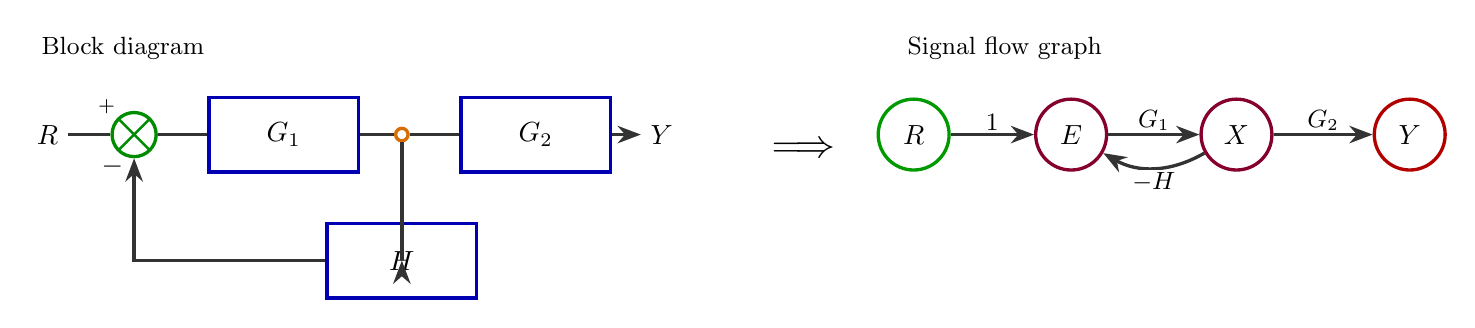
\begin{tikzpicture}
  % block diagram
  \node[note, anchor=west] at (0,2.9) {Block diagram};
  \node (r) at (0.2,1.8) {$R$};
  \node[sum] (s1) at (1.3,1.8) {};
  \node[block] (g1) at (3.2,1.8) {$G_1$};
  \node[tap] (tp) at (4.7,1.8) {};
  \node[block] (g2) at (6.4,1.8) {$G_2$};
  \node (y) at (8.0,1.8) {$Y$};
  \node[block] (h) at (4.7,0.2) {$H$};
  \draw[signal] (r) -- (s1) -- (g1) -- (tp) -- (g2) -- (y);
  \draw[signal] (tp) |- (h);
  \draw[signal] (h) -| node[pos=0.96, left] {$-$} (s1.south);
  \node[font=\scriptsize] at ($(s1)+(-0.35,0.35)$) {$+$};

  \node[font=\Large] at (9.8,1.6) {$\Longrightarrow$};

  % sfg
  \node[note, anchor=west] at (11.0,2.9) {Signal flow graph};
  \node[sfgsource] (rr) at (11.2,1.8) {$R$};
  \node[sfgnode] (e) at (13.2,1.8) {$E$};
  \node[sfgnode] (x) at (15.3,1.8) {$X$};
  \node[sfgsink] (yy) at (17.5,1.8) {$Y$};
  \draw[sfgedge] (rr) -- node[gain, above] {$1$} (e);
  \draw[sfgedge] (e) -- node[gain, above] {$G_1$} (x);
  \draw[sfgedge] (x) -- node[gain, above] {$G_2$} (yy);
  \draw[sfgedge, bend left=30] (x) to node[gain, below] {$-H$} (e);
\end{tikzpicture}
\end{document}
